\documentclass{article}
\usepackage[utf8]{inputenc}
\usepackage{tikz}
\usepackage{tkz-graph}
\usepackage{float}
\usepackage{amsmath}
\GraphInit[vstyle = Shade]

\title{Assignment 2}
\author{Jason Fantl, Jacob Tuttle}
\date{November 2019}

\begin{document}

\maketitle

\section{Theory vs. Practice}

3 reasons why asymptotic analysis may be misleading with respect to actual performance in practice:
\begin{itemize}
  \item Because asymptotic analysis ignores constants, it can lead to misrepresenting which algorithm is more efficient for specific situations. For example, if one algorithm runs in O(n) time and another runs in O($n^2$) time, you would assume the O(n) algorithm is more efficient. But if you also know that constants are included, and that the linear time algorithm would run in $10000n$ time, and the other in $n^2$ time, the more efficient algorithm depends on your input size, not just asymptotic time complexity.
  \item In practice there are always restrictions on both memory and time, and asymptotic analysis only considers how well an algorithm scales, not how well it will fit within the given conditions. This could lead to using an algorithm that scales very well but fails to complete the task at all within the available constraints. For example, if an algorithm were to rely on a large volume of memory access, when run on a computer with very efficient memory access techniques, these actions would have little effect on the runtime; however, if it were run on a device with much less efficient memory access, the execution time would balloon as a result that has nothing to do with the $O$ complexity.
  \item While asymptotic analysis will provide information about how the algorithm will behave in the abstract sense, it says nothing about how the code will run on a specific machine. Even if one were to run the algorithm on one machine, and use this data to extrapolate the runtimes for various input sizes, that information would mean nothing if the algorithm were run on another machine. The asymptotic runtime of an algorithm says very little about the true execution time for an algorithm, and it provides even less information when considering the differences of running on different machines.
\end{itemize}

Given a binary search tree with $1,000$ elements and a measured time of $5$ seconds to access one of those elements, we could use asymptotic analysis to predict how long it would take to find in element in a binary search tree with $10,000$ elements.
We know the time complexity of a searching in a binary search tree is $O(log(n))$. We can find the ratio of time it should take between different trees using this fact. The ratio of time between a tree with $1,000$ elements and a tree with $10,000$ should be $log_2(1,000)/log_2(10,000) = 0.75$. Using this calculation and the fact that the $1,000$ element tree took $5$ seconds, we predict it should take $\frac{5}{0.75} = 6.67$ seconds to find an element.

If the measured time of the two binary search trees doesn't match our prediction, here are three reasons why that might have happened:
\begin{itemize}
  \item Since $O$ only describes the highest order term, disregarding constants and lower order terms, one of these discarded terms may have been much larger than was initially considered. If one of these constants or lower order terms were to be quite large, increasing the input size could change the run time more significantly than calculations indicate.
  \item Depending on what form the input binary tree takes, the worst case time complexity of searching can be $O(n)$. It's possible the first execution, the $5$ second one, ran on an average or best case tree and the second execution ran on a worst case input. This would result in a much larger execution time since the worst case takes asymptotically more time than the average case.
  \item If the algorithm were run on different computers, then even if one were to run the same algorithm on the same tree, different run times could be produced. When run on a slower computer, this difference would be even more pronounced and could result in the difference between calculated and observed run times discussed in this problem.
\end{itemize}

\section{Graph Properties}


Definitions:
\begin{itemize}
\item Isomorphic: G1 = (V1, E1) is isomorphic to G2 = (V2, E2) if there is a
one-to-one and onto function $f : V1 \rightarrow V2$ such that
$(u, v) \in E1 \iff (f(u), f(v)) \in E2$
\item Completely connected: A graph is completely connected if there exists an edge between every pair of vertices.
\item One-to-One function: A function f is one-to-one if for all x and y f(x) = f(y) then x = y.
\item Onto function: A function f is onto if for all y in the range of f there exists an x such that f(x) = y
\end{itemize}

%Theorem: If two graphs A and B have the same number of nodes and are completely connected, they are isomorphic.

%Proof:
%We have a completely connected graph G1 = (V1, E1), and a completely connected graph G2 = (V2, E2) both with x vertices. We will label each vertex of graph G1 from V1 to Vx since it has x vertices. Then for each vertex, it has x edges since a completely connected graph connects every pair of vertices, and there are x vertices. For each edge edge coming out of vertex Vn, connecting to Vm, we will label that edge as En,m. Since G2 has the same number of vertices and is also completely connected, we will label all of its vertices and edges in the same exact way. Now there exists a simple function f which takes an edge or vertex and returns the same vertex or edge, that is f(u) = u and f(v) = v. This function is one-to-one since for all Pn and Qm where Pn and Qm are arbitrary vertices or edges, if f(Pn) = f(Qm) then Pn = Qm by the definition of f. f is also onto since for any value I in the range of f we pick a new value J = I, then f(J) = I by the definition of f. 

%To be continued \\

Theorem: If two graphs A and B have the same number of nodes and are completely connected, they are isomorphic. \\

Proof: Let $A$ and $B$ be two graphs that are completely connected and have the same number of nodes. By the definition of two completely connected graphs, we can define $A$ as a set of vertices $V_A$ labeled $a_1, a_2, \hdots a_n$ and a set of edges $E_A : (a_1, a_2), (a_1, a_3), \hdots (a_1, a_n), (a_2, a_3), (a_2, a_4), \hdots (a_2, a_n), \hdots (a_{n-1}, a_n)$. Likewise, $B$ is defined in a similar fashion with vertices $V_B : b_1, b_2, \hdots b_n$ and edges $E_B : (b_1, b_2), (b_1, b_3), \hdots (b_1, b_n), (b_2, b_3), (b_2, b_4), \hdots (b_2, b_n), \hdots (b_{n-1}, b_n)$. For these two graphs to be isomorphic, there must be a one-to-one and onto function $f: V1 \rightarrow V2$ such that $(u, v) \in E_A \iff (f(u), f(v)) \in E_B$ \\

If we can find this bijection, $f$, such that $(u, v) \in E_A \iff (f(u), f(v)) \in E_B$ then it will be shown that $A$ and $B$ are isomorphic. Let $f$ be defined as the function such that:
\begin{align*}
    f(a_1) &= b_1 \\
    f(a_2) &= b_2 \\
    &\vdots \\
    f(a_n) &= b_n
\end{align*}

$f$ is onto and one-to-one as we have defined it because every node in $V_A$ can be mapped by $f$ to a single corresponding node in $V_B$.

Using this function, it can be shown that every edge in $A$ corresponds to the same edge $(f(a_i), f(a_j)) = (b_i, b_j)$ for all $i, j \leq n$. Therefore, $A$ and $B$ are isomorphic. \\

% Old proof that is added 
%Theorem: If two graphs A and B are isomorphic they do not need to be completely connected.

%Proof: Let there be graphs G1 and G2 such that both have 3 vertices, called A1, B1, and C1 for G1, and A2, B2, and C2 for G2. Let G1 only have edges from A1 to B1 called AB1 and B1 to C1 called BC1, and let G2 only have edges from A2 to B2 called AB2 and B2 to C2 called BC2. Neither of these graphs are fully connected since there isn't an edge from A1 to C1 and there isn't an edge from A2 to C2. These graphs are isomorphic since the edge AB1 can be mapped to AB2 and BC1 mapped to BC2, and the edge and AB2 can be mapped to AB1 and BC2 mapped to BC1. This exhaustively finds a mapping between the sets of edges. By this example, we have found two graphs which are isomorphic and not fully connected, proving the theorem.*/

Theorem: If two graphs $A$ and $B$ are isomorphic, they do not need to be completely connected. \\

Proof: Let $A$ and $B$ be the graphs by Figure 1 and Figure 2 respectively and be defined as: 

\begin{align*}
    A &= (V_A, E_A) \\
    V_A &= \{a, b, c\} \\
    E_A &= \{(a, c), (c, b)\} \\
    B &= (V_B, E_B) \\
    V_B &= \{x, y, z\} \\
    E_B &= \{(x, y), (y, z)\}
\end{align*}

\begin{figure}[H]
    \centering
    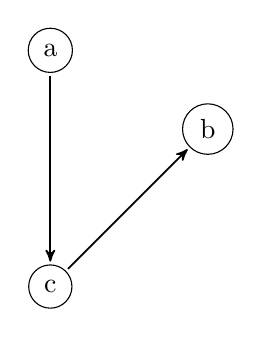
\begin{tikzpicture}[shorten >=1pt, auto, node distance=3cm]
    
    % draw nodes
    \foreach [count=\i] \x/\y/\t in {0/0/c, 0/3/a, 2/2/b}
        \node [circle, draw]
            (v\t) at (\x, \y) {\t};
            
    % draw edges
    \foreach \i/\j in {a/c, c/b}
        \draw (v\i) edge[post] (v\j);
    
    \end{tikzpicture}
    \caption{Graph $A$}
    \label{fig:graph_a}
\end{figure}
\begin{figure}[H]
    \centering
    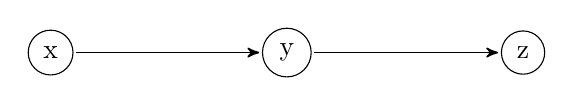
\begin{tikzpicture}[shorten >=1pt, auto, node distance=3cm]
    
    % draw nodes
    \foreach [count=\i] \x/\y/\t in {0/0/x, 3/0/y, 6/0/z}
        \node [circle, draw]
            (v\t) at (\x, \y) {\t};
            
    % draw edges
    \foreach \i/\j in {x/y, y/z}
        \draw (v\i) edge[post] (v\j);
    
    \end{tikzpicture}
    \caption{Graph $B$}
    \label{fig:graph_b}
\end{figure}
Let $f$ be a one-to-one and onto bijection from $A \rightarrow B$ such that:
\begin{align*}
    f(a) &= x \\
    f(b) &= z \\
    f(c) &= y
\end{align*}
Using the definitions above, it can be seen that all edges are mapped from $E_A$ to $E_B$ by $f$ and $f$ is one-to-one and onto from $A \rightarrow B$. Furthermore, in graph $A$ nodes $a$ and $b$ are not connected and in graph $B$ nodes $x$ and $z$ are not connected; therefore, the graphs are not completely connected. These graphs satisfy the theorem as two graphs that are isomorphic and not completely connected; therefore two graphs do not need to be completely connected to be isomorphic.

\section{Ford-Fulkerson --- Augmenting Paths}
Code solutions to this problem are provided in: \\ \texttt{Ford-Fulkerson\_Augmenting\_Paths.js}

\section{Ford-Fulkerson Algorithm }

Residual graph, iteration 1:

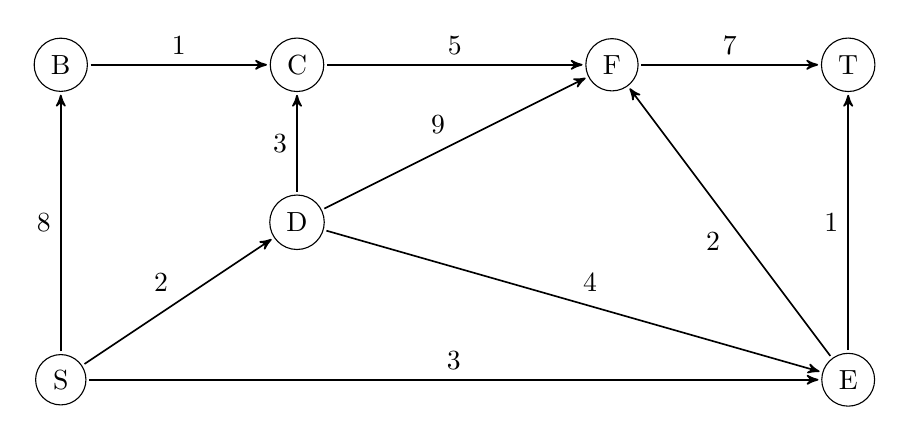
\begin{tikzpicture}[shorten >=1pt, auto, node distance=3cm]

   \foreach [count=\i] \x/\y/\t in {0/0/S, 0/4/B, 3/4/C, 3/2/D, 10/0/E, 7/4/F, 10/4/T}
     \node [circle,draw]
        (v\t) at (\x,\y) {\t};

   \foreach \i/\j/\t in {S/B/8, S/D/2, S/E/3, B/C/1, D/C/3, D/F/9, D/E/4, E/F/2, E/T/1, C/F/5, F/T/7}
    \draw (v\i) edge[post] node{\t} (v\j);
\end{tikzpicture}


Residual graph, iteration 2:

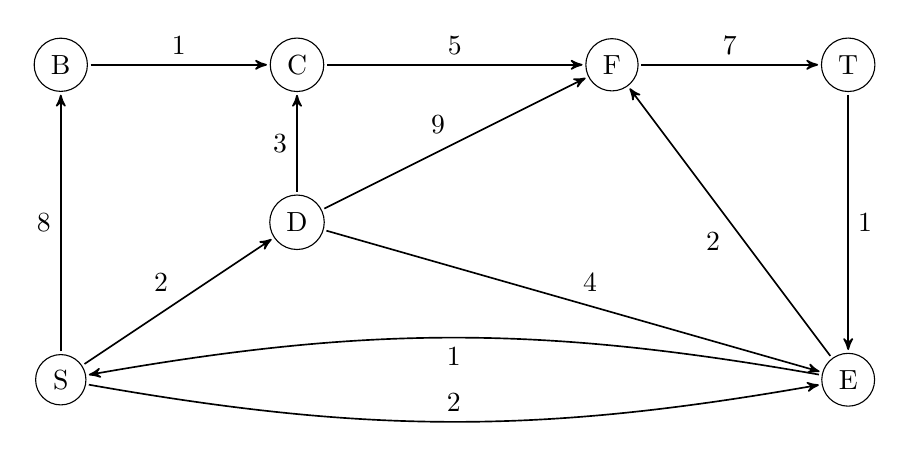
\begin{tikzpicture}[shorten >=1pt, auto, node distance=3cm]

   \foreach [count=\i] \x/\y/\t in {0/0/S, 0/4/B, 3/4/C, 3/2/D, 10/0/E, 7/4/F, 10/4/T}
     \node [circle,draw]
        (v\t) at (\x,\y) {\t};

    \foreach \i/\j/\t in {S/B/8, S/D/2, B/C/1, D/C/3, D/F/9, D/E/4, E/F/2, T/E/1, C/F/5, F/T/7}
        \draw (v\i) edge[post] node{\t} (v\j);
    \foreach \i/\j/\t in {S/E/2, E/S/1}
        \draw (v\i) edge[post, bend right=10] node{\t} (v\j);
    
\end{tikzpicture}

Residual graph, iteration 3:

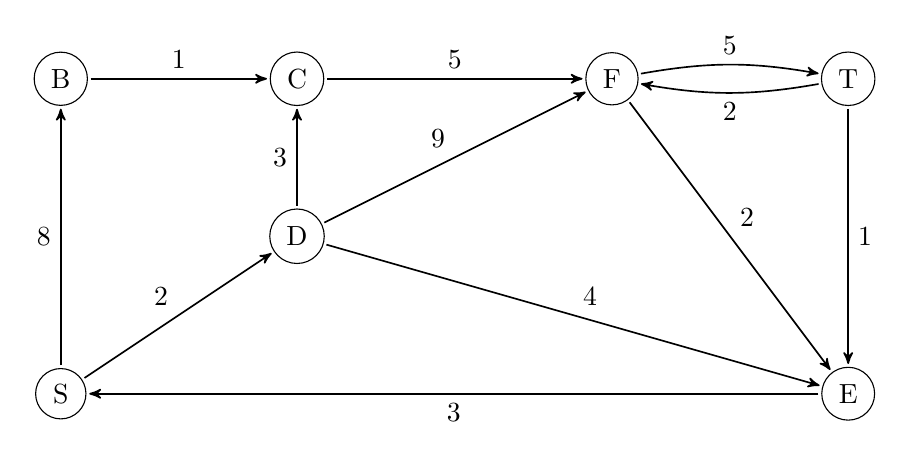
\begin{tikzpicture}[shorten >=1pt, auto, node distance=3cm]

   \foreach [count=\i] \x/\y/\t in {0/0/S, 0/4/B, 3/4/C, 3/2/D, 10/0/E, 7/4/F, 10/4/T}
     \node [circle,draw]
        (v\t) at (\x,\y) {\t};

    \foreach \i/\j/\t in {S/B/8, S/D/2, B/C/1, D/C/3, D/F/9, D/E/4, F/E/2, T/E/1, C/F/5, E/S/3}
        \draw (v\i) edge[post] node{\t} (v\j);
    \foreach \i/\j/\t in {F/T/5, T/F/2}
        \draw (v\i) edge[post, bend left=10] node{\t} (v\j);
    
\end{tikzpicture}

Residual graph, iteration 4:

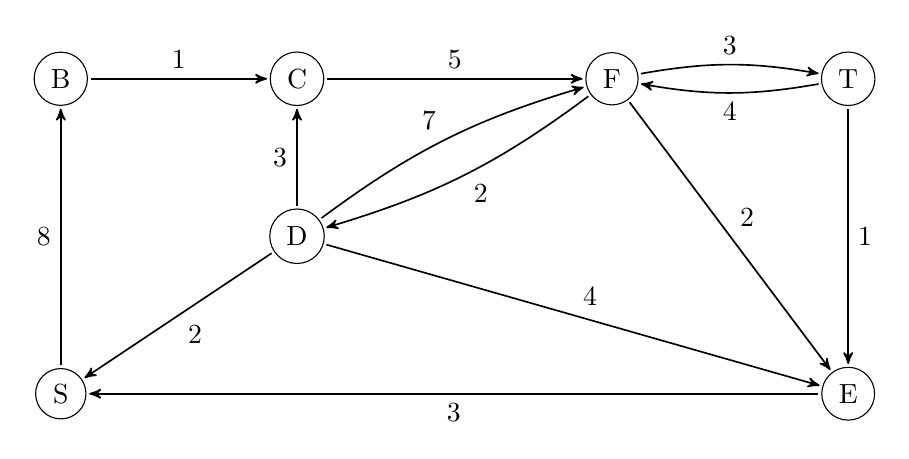
\begin{tikzpicture}[shorten >=1pt, auto, node distance=3cm]

   \foreach [count=\i] \x/\y/\t in {0/0/S, 0/4/B, 3/4/C, 3/2/D, 10/0/E, 7/4/F, 10/4/T}
     \node [circle,draw]
        (v\t) at (\x,\y) {\t};

    \foreach \i/\j/\t in {S/B/8, D/S/2, B/C/1, D/C/3, D/E/4, F/E/2, T/E/1, C/F/5, E/S/3}
        \draw (v\i) edge[post] node{\t} (v\j);
    \foreach \i/\j/\t in {F/T/3, T/F/4, D/F/7, F/D/2}
        \draw (v\i) edge[post, bend left=10] node{\t} (v\j);
    
\end{tikzpicture}

Residual graph, iteration 5:

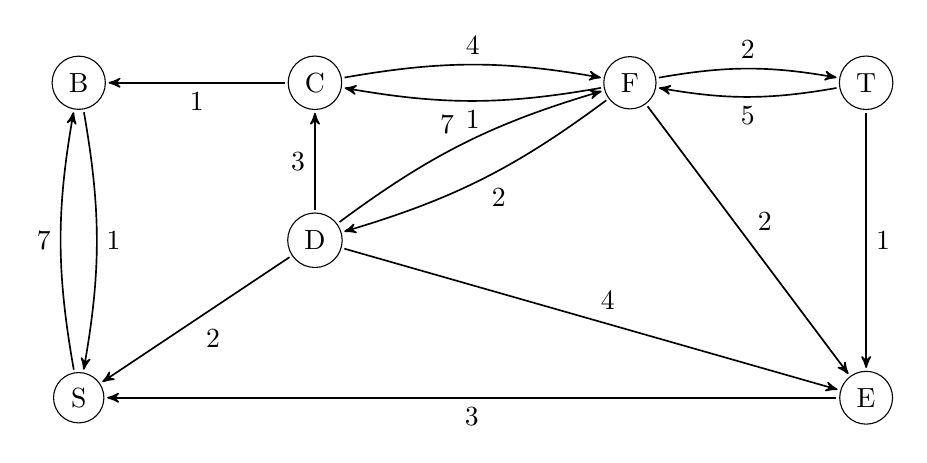
\begin{tikzpicture}[shorten >=1pt, auto, node distance=3cm]

   \foreach [count=\i] \x/\y/\t in {0/0/S, 0/4/B, 3/4/C, 3/2/D, 10/0/E, 7/4/F, 10/4/T}
     \node [circle,draw]
        (v\t) at (\x,\y) {\t};

    \foreach \i/\j/\t in {D/S/2, C/B/1, D/C/3, D/E/4, F/E/2, T/E/1, E/S/3}
        \draw (v\i) edge[post] node{\t} (v\j);
    \foreach \i/\j/\t in {S/B/7, B/S/1, C/F/4, F/C/1, F/T/2, T/F/5, D/F/7, F/D/2}
        \draw (v\i) edge[post, bend left=10] node{\t} (v\j);
    
\end{tikzpicture}

Original graph: Max flow of 6

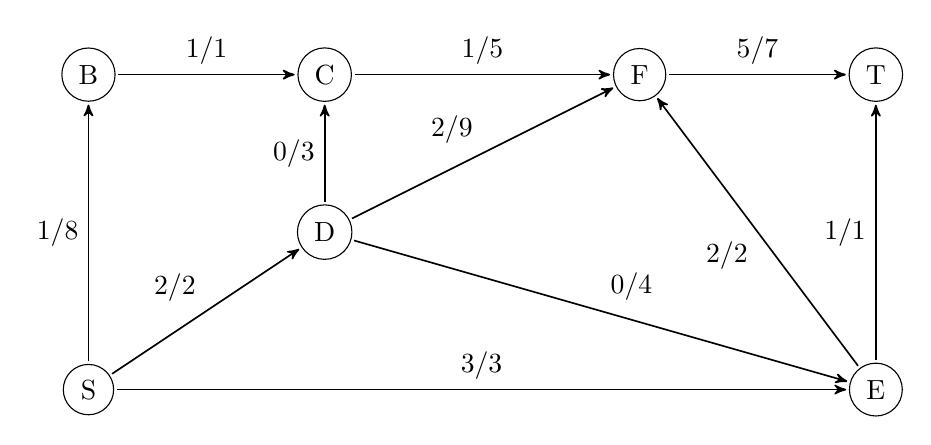
\begin{tikzpicture}[shorten >=1pt, auto, node distance=3cm]

   \foreach [count=\i] \x/\y/\t in {0/0/S, 0/4/B, 3/4/C, 3/2/D, 10/0/E, 7/4/F, 10/4/T}
     \node [circle,draw]
        (v\t) at (\x,\y) {\t};

    \foreach \i/\j/\f/\t in {S/B/1/8, S/D/2/2, S/E/3/3, B/C/1/1, D/C/0/3, D/F/2/9, D/E/0/4, E/F/2/2, E/T/1/1, C/F/1/5, F/T/5/7}
        \draw (v\i) edge[post] node{\f/\t} (v\j);

\end{tikzpicture}

\section{Kruskal’s Algorithm }
Minimum spanning tree, iteration 1:

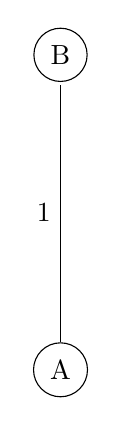
\begin{tikzpicture}[shorten >=1pt, auto, node distance=3cm]

   \foreach [count=\i] \x/\y/\t in {0/0/A, 0/4/B}
     \node [circle,draw]
        (v\t) at (\x,\y) {\t};

    \foreach \i/\j/\t in {A/B/1}
        \draw (v\i) edge node{\t} (v\j);
    
\end{tikzpicture}

Minimum spanning tree, iteration 2:

\begin{tikzpicture}[shorten >=1pt, auto, node distance=3cm]

   \foreach [count=\i] \x/\y/\t in {0/0/A, 0/4/B, 10/0/E, 7/4/F}
     \node [circle,draw]
        (v\t) at (\x,\y) {\t};

    \foreach \i/\j/\t in {A/B/1, E/F/2}
        \draw (v\i) edge node{\t} (v\j);
    
\end{tikzpicture}

Minimum spanning tree, iteration 3:

\begin{tikzpicture}[shorten >=1pt, auto, node distance=3cm]

   \foreach [count=\i] \x/\y/\t in {0/0/A, 0/4/B, 3/4/C, 3/2/D, 10/0/E, 7/4/F}
     \node [circle,draw]
        (v\t) at (\x,\y) {\t};

    \foreach \i/\j/\t in {A/B/1, E/F/2, A/E/3, D/C/3}
        \draw (v\i) edge node{\t} (v\j);
    
\end{tikzpicture}

Minimum spanning tree, iteration 4:

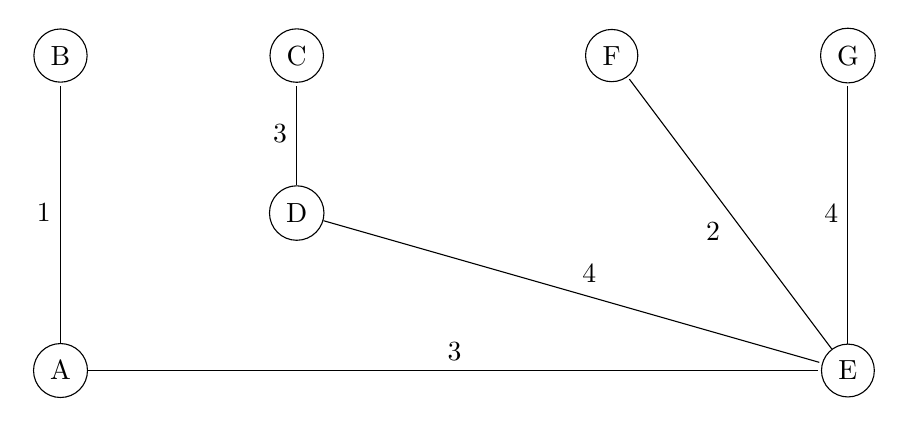
\begin{tikzpicture}[shorten >=1pt, auto, node distance=3cm]

   \foreach [count=\i] \x/\y/\t in {0/0/A, 0/4/B, 3/4/C, 3/2/D, 10/0/E, 7/4/F, 10/4/G}
     \node [circle,draw]
        (v\t) at (\x,\y) {\t};

    \foreach \i/\j/\t in {A/B/1, E/F/2, A/E/3, D/C/3, E/G/4, D/E/4}
        \draw (v\i) edge node{\t} (v\j);
    
\end{tikzpicture}

Minimum spanning tree, iteration 5:

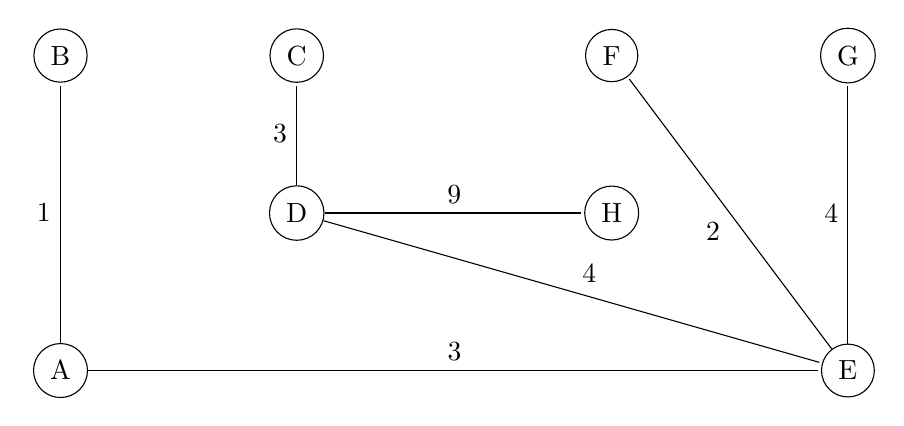
\begin{tikzpicture}[shorten >=1pt, auto, node distance=3cm]

   \foreach [count=\i] \x/\y/\t in {0/0/A, 0/4/B, 3/4/C, 3/2/D, 10/0/E, 7/4/F, 10/4/G, 7/2/H}
     \node [circle,draw]
        (v\t) at (\x,\y) {\t};

    \foreach \i/\j/\t in {A/B/1, E/F/2, A/E/3, D/C/3, E/G/4, D/E/4, D/H/9}
        \draw (v\i) edge node{\t} (v\j);
    
\end{tikzpicture}
\end{document}
